\chapter{Diseño e implementación} % Main chapter title

\label{Chapter3} % Change X to a consecutive number; for referencing this chapter elsewhere, use \ref{ChapterX}

Este capítulo aborda el proceso de construcción del sistema de recomendación, desde la concepción de la solución hasta su materialización en un entorno operativo. Se presentan las principales decisiones de diseño, el tratamiento de los datos y las técnicas empleadas para generar las recomendaciones, así como los lineamientos seguidos para asegurar que la propuesta resulte escalable, reproducible y alineada con los objetivos del negocio.

%----------------------------------------------------------------------------------------

\section{Diseño de solución}

El sistema de recomendación se diseñó con el objetivo de estimar la afinidad entre clientes y productos en un entorno caracterizado por alta escala, heterogeneidad de perfiles y rotación constante del portafolio. El diseño de la solución se apoyó en una arquitectura en capas que permite integrar diversas fuentes de datos, transformarlas en estructuras analíticas consistentes, entrenar modelos capaces de capturar relaciones complejas y, finalmente, desplegar las recomendaciones en un flujo operativo estable y reproducible.

La primera capa corresponde a la ingestión de datos, instancia en la que se integran registros transaccionales, interacciones digitales y atributos contextuales. Los datos transaccionales reflejan las compras efectivas realizadas en distintos horizontes temporales, lo que aporta evidencia directa sobre las preferencias observadas. Las interacciones digitales, en cambio, ofrecen señales implícitas de interés a partir de búsquedas, visualizaciones de productos o modificaciones en el carrito. Finalmente, los atributos contextuales caracterizan tanto a los clientes, mediante variables asociadas a su canal de comercialización, localización o tamaño, como a los productos, a partir de propiedades como marca, categoría o segmento.

La segunda capa se orienta a la preparación de los datos. En esta etapa se construyen las matrices de interacciones cliente–producto y se generan representaciones temporales que permiten capturar la dinámica de la demanda. Asimismo, se aplican técnicas de tratamiento de valores faltantes y de codificación de atributos categóricos, con el fin de asegurar consistencia y compatibilidad entre las distintas fuentes. El resultado de este proceso es un conjunto de estructuras homogéneas que sientan las bases para la etapa de modelado.

El modelado constituye la tercera capa de la arquitectura. En este punto se combinan distintos enfoques con el fin de maximizar la capacidad predictiva y superar las limitaciones de cada técnica individual. El filtrado colaborativo implícito, implementado a través de factorización matricial con el método ALS, permite capturar patrones latentes a partir de historiales de compra extensos. Los modelos basados en contenido complementan este enfoque al aprovechar descripciones de clientes y productos, y ofrecen una alternativa frente al problema del arranque en frío. Adicionalmente, se exploran modelos híbridos y de aprendizaje profundo capaces de integrar simultáneamente señales transaccionales y digitales, y de modelar relaciones no lineales entre las variables.

Finalmente, la capa de despliegue asegura la integración del motor de recomendación en el ecosistema tecnológico de la empresa. El pipeline resultante genera listas de productos priorizados para cada cliente, incorpora mecanismos de versionado y monitoreo de modelos, y permite evaluar su desempeño en forma continua. De este modo, la solución se diseñó no solo para alcanzar precisión en la generación de recomendaciones, sino también para garantizar escalabilidad, reproducibilidad y adaptabilidad frente a la evolución del portafolio y a los cambios en los objetivos estratégicos.

La arquitectura de la solución se representa en la figura \ref{fig:arquitectura}. Allí se observa el flujo general del sistema, desde la integración de datos hasta la generación de recomendaciones. El diagrama sintetiza los módulos principales y sus interacciones, y ofrece una visión global que facilita comprender cómo se organiza el motor de afinidad.

\begin{figure}[H]
  \centering
  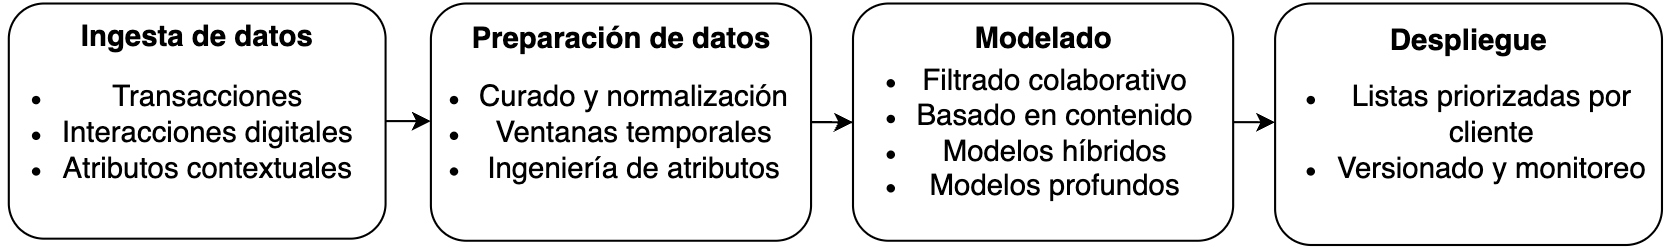
\includegraphics[width=0.9\textwidth]{Figures/Arquitectura.png}
  \caption{Arquitectura de alto nivel del sistema de recomendación.}
  \label{fig:arquitectura}
\end{figure}

%----------------------------------------------------------------------------------------

\section{Preparación de los datos}

La preparación de los datos se centró en transformar las distintas fuentes disponibles en insumos consistentes y comparables para el entrenamiento de los modelos de recomendación. El proceso partió de tres conjuntos principales de información: registros transaccionales, eventos digitales generados en la aplicación y atributos contextuales de clientes y productos. La combinación de estas fuentes permitió construir una representación integral de la relación cliente–producto, en la que se entrelazan tanto preferencias explícitas como señales implícitas de interés.

Los registros transaccionales se encontraban a nivel de operación individual, con granularidad diaria y asociados a identificadores de cliente, producto, cantidad y monto. Este tipo de información es particularmente relevante en entornos de consumo masivo B2B, donde suele observarse una fuerte concentración de las compras en un subconjunto reducido de productos y clientes. De manera preliminar, se advierte un patrón cercano a la regla de Pareto \cite{BOOK:Koch1998}, un pequeño grupo de marcas concentra la mayor parte del volumen mientras que muchos otros artículos registran ventas esporádicas. Esta característica, común en el sector, anticipa la necesidad de abordar los sesgos hacia productos de alta rotación en etapas posteriores del análisis.

Los eventos digitales, por su parte, se encontraban a nivel de interacción, con registros de búsquedas, visualizaciones, adiciones y remociones en el carrito, y clics en promociones. Estos datos permiten capturar señales tempranas de interés que no siempre se traducen en transacciones. No obstante, su naturaleza los hace sensibles al ruido: interacciones aisladas, comportamientos exploratorios o promociones masivas pueden generar señales que no representan un patrón estable. En consecuencia, aunque aportan cobertura y diversidad, requieren una interpretación cuidadosa para evitar que se sobreestimen comportamientos circunstanciales.

Finalmente, los atributos contextuales ofrecieron información complementaria a nivel de cliente y producto. En el caso de los clientes, la granularidad fue de punto de venta, con variables que reflejan diferencias de canal, localización o tamaño, factores que suelen condicionar significativamente las decisiones de compra. En el caso de los productos, los atributos de marca, segmento, envase o rango de precio permiten distinguir entre artículos de consumo masivo y aquellos de carácter más selectivo, lo que introduce heterogeneidad que no siempre se refleja en los registros transaccionales.

La integración de estas fuentes en un repositorio unificado aseguró la compatibilidad de identificadores y la alineación temporal de los registros, lo que habilitó su uso conjunto en el análisis. Las primeras observaciones sugieren un escenario donde coexisten concentración de la demanda en pocos productos y clientes, señales digitales útiles pero ruidosas y una marcada diversidad contextual. Estos fenómenos, característicos del consumo masivo B2B, definen los ejes que serán explorados en mayor detalle durante el análisis exploratorio y que posteriormente condicionarán las decisiones de ingeniería de atributos y modelado.

%----------------------------------------------------------------------------------------

\section{Análisis exploratorio de los datos}

El análisis exploratorio constituye una etapa fundamental para comprender la estructura y los patrones subyacentes en la información disponible antes de su utilización en modelos de recomendación. Su objetivo es identificar distribuciones, tendencias y relaciones entre variables que permitan caracterizar el comportamiento de los clientes y del portafolio de productos, así como anticipar posibles limitaciones o sesgos que afecten el desempeño de los algoritmos.

En esta sección se examinan distintas dimensiones de los datos, e incluye la concentración de clientes y productos, la diversidad de los portafolios de compra, las correlaciones entre variables transaccionales y digitales, y la presencia de sesgos asociados a la popularidad.Este análisis preliminar no solo proporciona una visión descriptiva del conjunto de datos, sino que también orienta decisiones posteriores de ingeniería de atributos y diseño de modelos, al revelar qué señales resultan más informativas y qué fenómenos requieren un tratamiento específico.

\subsection{Curvas de concentración de clientes y productos}

El análisis de concentración constituye un paso clave para comprender la distribución del consumo en entornos de negocio masivo. La figura \ref{fig:concentracion_productos} muestra la curva de concentración de productos, donde se observa que un reducido conjunto concentra la mayor parte del volumen total. En particular, el 20\% de los productos explica cerca del 90\% de las ventas acumuladas, mientras que el resto conforma una extensa cola larga con niveles de rotación significativamente menores. Este comportamiento coincide con la ley de Pareto o principio 80/20 \cite{BOOK:Koch1998}, ampliamente documentado en mercados de consumo masivo, donde la dinámica competitiva se organiza en torno a un pequeño núcleo de artículos de alta popularidad y una mayoría de baja incidencia \cite{BOOK:Anderson2006}.

\begin{figure}[htpb]
	\centering
	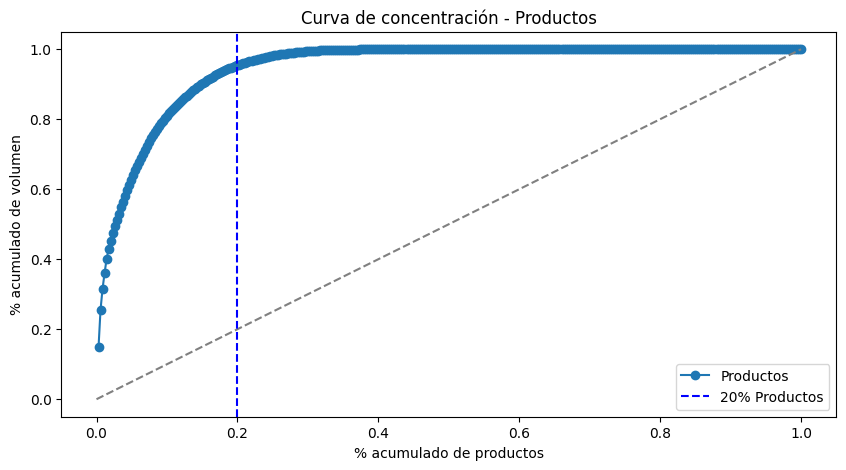
\includegraphics[scale=.55]{./Figures/concentracion_productos.png}
	\caption{Concentración de productos en el portafolio.}
	\label{fig:concentracion_productos}
\end{figure}

De manera análoga, la figura \ref{fig:concentracion_clientes} refleja la concentración del consumo en la base de clientes. Los resultados indican que cerca del 20\% de los puntos de venta generan alrededor del 80\% del volumen total, lo que pone de manifiesto la existencia de clientes estratégicos que concentran gran parte de la demanda. Esta distribución desigual plantea desafíos relevantes para el diseño de sistemas de recomendación, ya que las señales provenientes de clientes de alto volumen tienden a dominar los modelos, lo que genera sesgos hacia productos y comportamientos mayoritarios.

\begin{figure}[htpb]
	\centering
	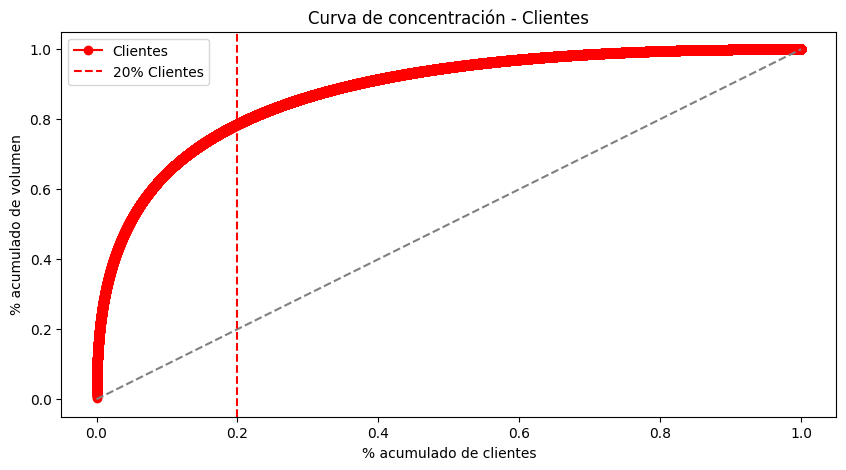
\includegraphics[scale=.55]{./Figures/concentracion_clientes.png}
	\caption{Concentración de clientes.}
	\label{fig:concentracion_clientes}
\end{figure}

La evidencia empírica confirma así que tanto el portafolio de productos como la base de clientes presentan fuertes patrones de concentración. En consecuencia, un motor de recomendación que busque maximizar su impacto no solo debe capturar la afinidad entre clientes y productos más relevantes, sino también considerar mecanismos que favorezcan la diversidad y la exploración de la cola larga. Esta perspectiva resulta fundamental para equilibrar la explotación de los artículos de mayor rotación con la exposición de productos menos populares, lo que alinea los objetivos de negocio con la mejora de la experiencia del cliente.

\subsection{Patrones de diversidad en el portafolio}

El análisis de la diversidad en el portafolio de productos por cliente permite comprender la amplitud y heterogeneidad de los hábitos de consumo. La figura \ref{fig:hist_diversidad} muestra la distribución del número de productos distintos adquiridos por cliente en un mes. Los resultados evidencian que la mayoría de los puntos de venta concentra su demanda en un conjunto reducido de referencias, mientras que un número menor incorpora una mayor amplitud de marcas y presentaciones. Esta asimetría confirma la coexistencia de clientes de bajo rango de exploración con otros de portafolio más diversificado.

\begin{figure}[htpb]
	\centering
	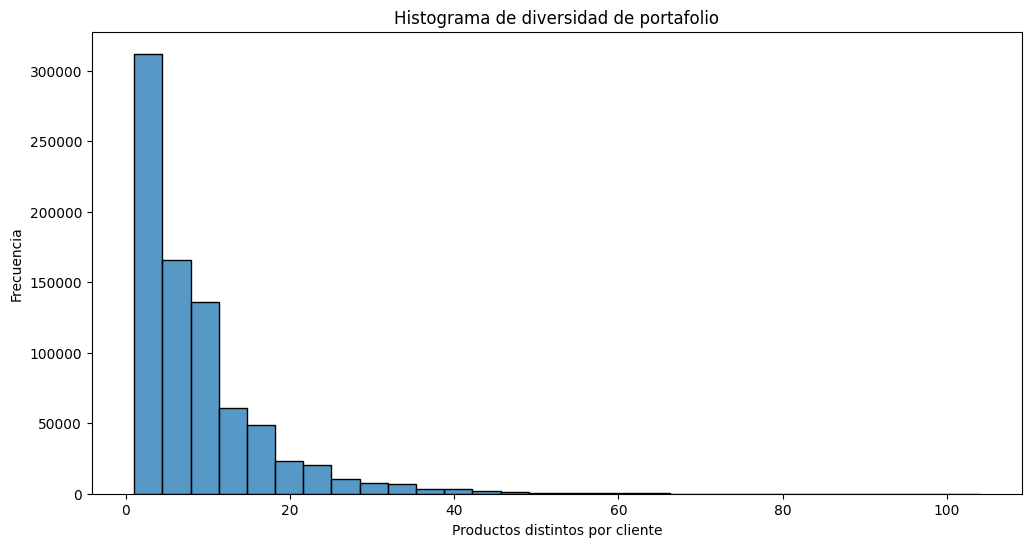
\includegraphics[scale=.55]{./Figures/hist_diversidad.png}
	\caption{Histograma de diversidad de portafolio: número de productos distintos por cliente.}
	\label{fig:hist_diversidad}
\end{figure}

Las diferencias se acentúan al segmentar por canal comercial, como se puede apreciar en la figura \ref{fig:boxplot_diversidad}. En este caso, se observa que los autoservicios tienden a manejar un surtido más amplio de productos en comparación con kioscos y tiendas tradicionales, lo que refleja el rol que cada formato cumple dentro de la red de distribución. Este hallazgo es consistente con la literatura en consumo masivo, que indica que la variedad de portafolio suele estar asociada a factores estructurales como el tamaño del punto de venta y la frecuencia de reposición \cite{BOOK:Kotler2017}.

\begin{figure}[htpb]
	\centering
	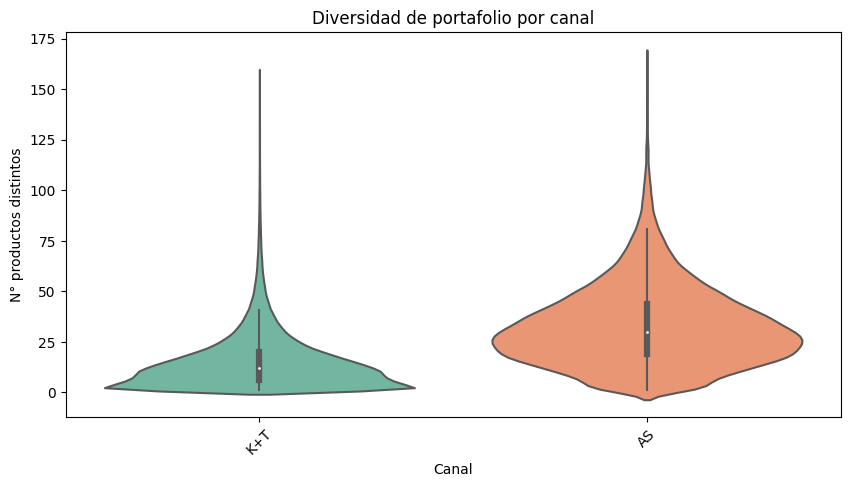
\includegraphics[scale=.55]{./Figures/boxplot_diversidad_canal.png}
	\caption{Diversidad de portafolio segmentada por canal comercial.}
	\label{fig:boxplot_diversidad}
\end{figure}

La figura \ref{fig:log_log_plot} ilustra el fenómeno de concentración extrema en la demanda, donde unos pocos productos acumulan la mayoría de los pedidos mientras que la gran mayoría registra volúmenes marginales. Para representar este patrón se utiliza un \textit{log–log plot}, en el cual tanto el ranking de los productos como su número total de pedidos se expresan en escala logarítmica. Esta transformación permite visualizar con mayor claridad distribuciones de tipo cola larga, que en escalas lineales suelen quedar ocultas por la presencia de artículos extremadamente populares. El gráfico muestra una pendiente decreciente que confirma la existencia de este comportamiento: un reducido conjunto de productos concentra un volumen muy elevado, mientras que el resto se distribuye en la larga cola de baja rotación.

Este patrón no solo refuerza la evidencia presentada en las curvas de concentración, sino que además resalta un sesgo estructural que enfrenta cualquier sistema de recomendación en entornos de consumo masivo. Al entrenarse sobre datos históricos, los modelos tienden de manera natural a privilegiar los productos más populares, lo que reproduce el sesgo de popularidad y reduce la diversidad de las sugerencias. Este fenómeno señala la tensión entre explotación de productos estrella y exploración de la cola larga \cite{BOOK:Celma2010}. En este contexto, el desafío consiste en diseñar mecanismos que permitan balancear ambos extremos, de modo que se garantice relevancia sin sacrificar diversidad ni cobertura.

\begin{figure}[htpb]
	\centering
	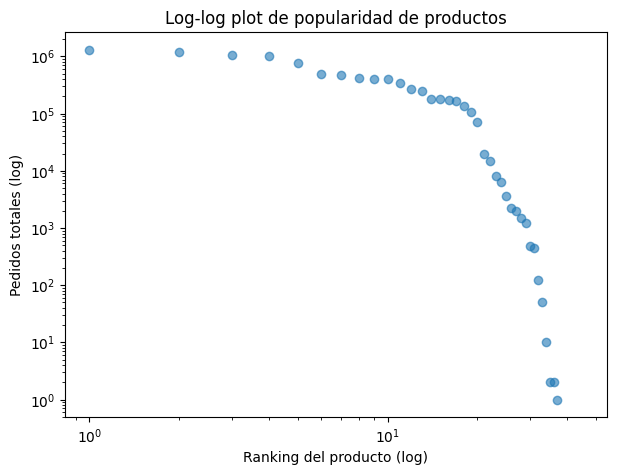
\includegraphics[scale=.6]{./Figures/log_log_plot.png}
	\caption{\textit{Log–log plot} de la popularidad de productos.}
	\label{fig:log_log_plot}
\end{figure}

El análisis de co-ocurrencia entre los productos más relevantes, presentado en la figura \ref{fig:heatmap_coocurrencia}, revela patrones de complementariedad en la demanda. Determinadas marcas y presentaciones tienden a aparecer de manera conjunta en los carritos de compra, lo que sugiere asociaciones naturales que pueden ser aprovechadas por un motor de recomendación. Estos resultados refuerzan la importancia de capturar no solo la popularidad individual de cada producto, sino también las relaciones de afinidad que emergen a nivel de portafolio.

\begin{figure}[htpb]
	\centering
	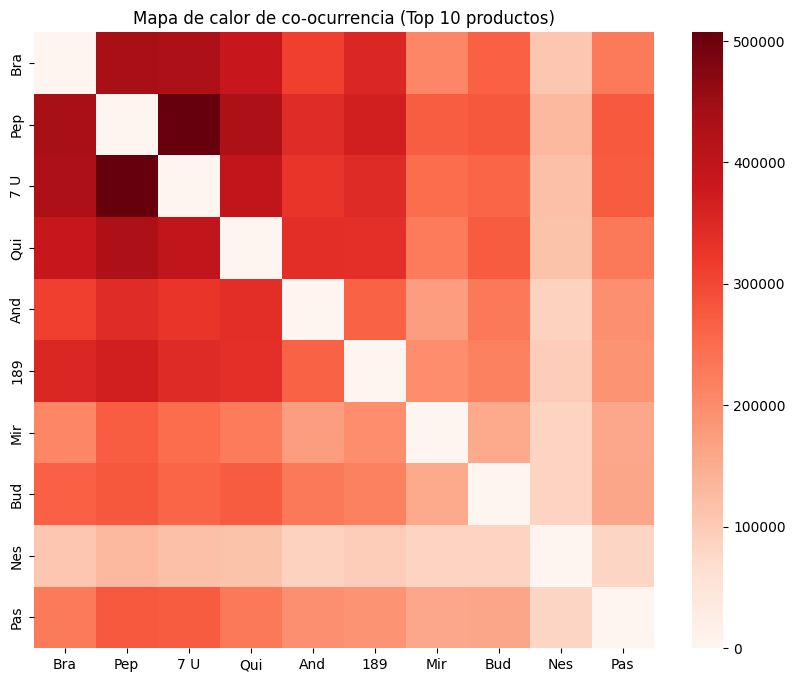
\includegraphics[scale=.45]{./Figures/heatmap_coocurrencia.png}
	\caption{Mapa de calor de co-ocurrencia entre los 10 productos más relevantes.}
	\label{fig:heatmap_coocurrencia}
\end{figure}

\subsection{Correlaciones entre variables transaccionales y digitales}

El análisis de correlaciones busca identificar hasta qué punto las señales digitales anticipan comportamientos de compra y, en consecuencia, evaluar su potencial como insumos predictivos. Con el fin de evaluar la relación entre interacciones digitales y transacciones, se construyó una matriz de correlación entre las principales variables del conjunto de datos, observada en la figura \ref{fig:heatmap_corr}. 

\begin{figure}[htpb]
	\centering
	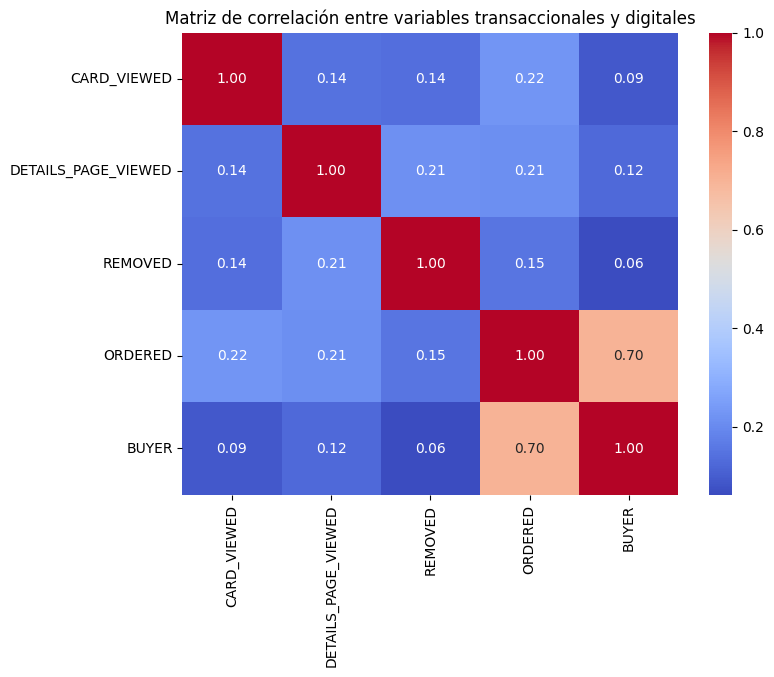
\includegraphics[scale=.55]{./Figures/heatmap_corr.png}
	\caption{Matriz de correlación entre variables transaccionales y digitales.}
	\label{fig:heatmap_corr}
\end{figure}

Los resultados muestran una correlación elevada entre \texttt{ORDERED} y \texttt{BUYER} ($r=0.70$), coherente con el hecho de que ambas variables reflejan distintos aspectos de la misma dimensión de compra. En contraste, las correlaciones de las señales digitales con las variables de compra resultan positivas pero de menor magnitud: \texttt{CARD\_VIEWED} y \texttt{DETAILS\_PAGE\_VIEWED} muestran coeficientes bajos, lo que indica que la exposición y exploración de productos acompaña el proceso de compra, aunque no lo determina. La variable \texttt{REMOVED} presenta la relación más débil, lo que sugiere que los eventos de descarte contienen información ruidosa y limitada respecto de la propensión a comprar.

La correlación contemporánea entre interacciones digitales y compras confirma que las transacciones pasadas siguen siendo el principal indicador de comportamiento, mientras que las señales digitales aportan evidencia complementaria que, si bien débil de manera aislada, resulta relevante al integrarse en un modelo híbrido.

Con el fin de explorar la capacidad predictiva de estas variables, se calculó la correlación de cada una con la compra del mismo cliente–producto en el mes siguiente. Los resultados, en la figura \ref{fig:corr_prox_mes},  muestran que las transacciones pasadas (\texttt{BUYER}, \texttt{ORDERED}) son los predictores más fuertes, aunque las señales digitales también aportan información incremental. En particular, la variable \texttt{CARD\_VIEWED} presenta un coeficiente relevante, lo que respalda la hipótesis de que la exposición reiterada a un producto incrementa la probabilidad de recompra.

\begin{figure}[htpb]
	\centering
	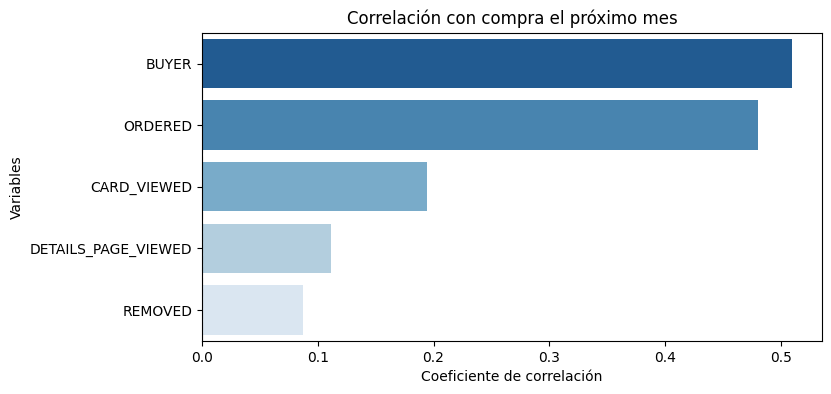
\includegraphics[scale=.5]{./Figures/corr_prox_mes.png}
	\caption{Correlación de variables con la compra en el mes siguiente.}
	\label{fig:corr_prox_mes}
\end{figure}

Finalmente, se evaluó la tasa de recompra según la combinación de señales observadas en meses previos, en la tabla \ref{tab:tasa_recompra}. Los clientes que registran tanto interacción como transacción presentan la mayor tasa de recompra (58,8\%), seguidos por aquellos con solo órdenes (44,1\%). En contraste, quienes solo exhiben interacciones digitales alcanzan un nivel considerablemente menor (17,6\%), incluso por debajo del grupo sin ningún registro previo (28,3\%). Este resultado sugiere que las interacciones aisladas no constituyen un predictor confiable de recompra, sino que tienden a reflejar un interés superficial que rara vez se traduce en pedidos. En cambio, la combinación de transacciones previas con señales digitales se confirma como el escenario de mayor poder explicativo, ya que aprovecha la solidez de la evidencia transaccional y, al mismo tiempo, permite mejorar la capacidad de anticipar comportamientos futuros en casos donde no existen registros abundantes de compra.

\begin{table}[h]
	\centering
	\caption[Tasa de recompra por combinación de señales]{Tasa de recompra según la combinación de señales previas.}
	\begin{tabular}{l c}    
		\toprule
		\textbf{Grupo}     & \textbf{Tasa de recompra}\\
		\midrule
		Interacción y orden & 58.79 \% \\
		Solo orden & 44.05 \% \\
		Ninguno & 28.30 \% \\
		Solo interacción & 17.64 \% \\
		\bottomrule
		\hline
	\end{tabular}
	\label{tab:tasa_recompra}
\end{table}

\subsection{Observaciones preliminares del análisis exploratorio}

El análisis exploratorio permitió identificar una serie de patrones que resultan fundamentales para orientar el diseño del motor de recomendación. En primer lugar, se confirmó que tanto el portafolio de productos como la base de clientes presentan fuertes niveles de concentración: un reducido conjunto explica la mayor parte del volumen, mientras que la mayoría se distribuye en una extensa cola larga de baja rotación. Este comportamiento introduce un sesgo hacia popularidad que los modelos deben manejar para no sacrificar diversidad \cite{BOOK:Anderson2006}.

En segundo lugar, se observó que la diversidad en los portafolios de compra varía según el tipo de cliente, con autoservicios que incorporan un surtido más amplio en comparación con kioscos y tiendas tradicionales. Además, los análisis de co-ocurrencia revelaron asociaciones frecuentes entre ciertos productos, lo que sugiere la existencia de complementariedades que pueden ser aprovechadas en la generación de recomendaciones.  

En tercer lugar, el estudio de correlaciones entre variables digitales y transaccionales mostró que, si bien las transacciones pasadas constituyen el predictor más sólido de comportamiento, las señales digitales aportan información incremental y se vuelven especialmente relevantes en escenarios de arranque en frío. La evaluación de tasas de recompra confirmó que la combinación de interacciones y compras pasadas es la fuente más robusta de predicción, mientras que las interacciones aisladas presentan un valor explicativo limitado.  

En conjunto, estos hallazgos proporcionan una primera validación de la hipótesis central: la integración de señales transaccionales y digitales, complementadas con atributos contextuales, resulta clave para capturar la heterogeneidad del consumo y diseñar un motor de recomendación capaz de balancear precisión, diversidad y cobertura.

%----------------------------------------------------------------------------------------

\section{Ingeniería de atributos}

La ingeniería de atributos busca transformar los datos en representaciones que los algoritmos de recomendación puedan utilizar de manera efectiva. Más que un proceso técnico de limpieza o transformación, implica decidir cómo capturar las relaciones entre clientes y productos para que el modelo cuente con señales relevantes al momento de aprender.

En un entorno B2B de consumo masivo, estas decisiones resultan especialmente importantes. La concentración de la demanda en pocos productos, la rotación frecuente del portafolio y la existencia de clientes sin historial son factores que obligan a diseñar atributos que reflejen esa complejidad. Para ello se definieron distintas ventanas temporales de observación, se combinaron transacciones con interacciones digitales y se incorporaron características contextuales que enriquecen la representación final.

También se aplicaron técnicas de agregación, codificación y normalización para equilibrar las variables y evitar que los productos más populares concentren toda la señal. El resultado es una matriz cliente–producto adecuada para algoritmos como ALS o LightFM, capaz de capturar patrones de afinidad y ofrecer recomendaciones más precisas.

\subsection{Ventanas temporales de datos}
Uno de los primeros aspectos a definir en la ingeniería de atributos es la ventana temporal sobre la que se mide el comportamiento de los clientes. La dinámica de compra en el canal B2B de consumo masivo no es homogénea: algunos puntos de venta realizan pedidos de manera semanal, mientras que otros concentran sus compras una vez al mes o incluso con menor frecuencia. Capturar estas diferencias requiere observar la información en distintos horizontes.

Para este trabajo se construyeron indicadores en tres escalas: corto plazo definido como un mes, mediano plazo correspondiente a tres meses y largo plazo equivalente a seis meses. La ventana de un mes refleja comportamientos inmediatos y ayuda a identificar tendencias recientes, como la adopción de un producto nuevo o la respuesta a una promoción puntual. La ventana de tres meses suaviza la volatilidad y permite reconocer patrones de consumo más estables. Finalmente, la de seis meses ofrece una visión de mayor persistencia, útil para productos de baja rotación o con fuerte estacionalidad.

El uso combinado de estas ventanas facilita que el modelo integre señales de distinto alcance temporal \cite{BOOK:Xiang2010, ARTICLE:Koren2010}, lo que equilibra la sensibilidad a cambios recientes con la estabilidad de patrones históricos. Así, un cliente que dejó de comprar un producto en el último mes pero que lo consumía de manera regular en períodos anteriores puede ser identificado de forma diferente a uno que nunca lo incorporó a su portafolio. De esta manera, se evita que las recomendaciones se basen únicamente en la foto más reciente y se logra un balance entre actualidad y consistencia histórica.

\subsection{Agregación de características}

Una vez definidas las variables de interés, fue necesario condensar la información en indicadores que representen de manera clara el comportamiento de cada cliente frente a cada producto. En las transacciones se calcularon medidas como el número total de órdenes, el volumen acumulado y la participación relativa de cada producto en el portafolio del cliente \cite{ARTICLE:Adomavicius2005}.

Las interacciones digitales se resumieron en recuentos de eventos significativos, tales como visualizaciones de producto, adiciones o remociones en el carrito y respuestas a promociones. Este tipo de métricas permiten obtener una señal cuantitativa de interés que complementa la evidencia proveniente de las compras efectivas \cite{BOOK:Ricci2015}.

Además, se incorporaron características contextuales tanto del lado del cliente como del producto. Para los clientes se consideraron variables como canal comercial, localización geográfica y tamaño del punto de venta. Para los productos, atributos como marca, segmento, envase y rango de precio \cite{BOOK:Aggarwal2016}. Estas propiedades enriquecen la caracterización de cada par cliente–producto y permiten capturar heterogeneidades relevantes para el sistema de recomendación.

El resultado es un conjunto de variables agregadas que sintetizan de manera equilibrada la información transaccional, digital y contextual, lo que conforma un insumo más robusto y manejable para la construcción de la matriz cliente–producto.

\subsection{Codificación de variables categóricas}

El conjunto de atributos contextuales incluyó variables de naturaleza categórica, tales como canal comercial, región geográfica, segmento de producto, marca o tipo de envase. Para que estas variables pudieran ser utilizadas en los algoritmos de recomendación fue necesario transformarlas en representaciones numéricas que preservaran su información.

En casos de variables con gran número de categorías, como la marca o el punto de venta, se aplicaron criterios de reducción para evitar una explosión dimensional. Las categorías de baja frecuencia se reagruparon en clases residuales, lo que garantizó que la codificación reflejara solo valores con suficiente representación en los datos. Este enfoque reduce la dispersión y mejora la estabilidad del entrenamiento, al tiempo que mantiene la capacidad de capturar patrones relevantes.

La estrategia aplicada fue la indexación de categorías \cite{BOOK:Ricci2015}, que asigna a cada valor un identificador numérico único dentro de su variable. De esta forma, un producto perteneciente a un determinado segmento o una venta registrada en un canal específico quedan representados de manera consistente.

Se obtuvo un conjunto de variables categóricas estandarizadas y codificadas, listas para integrarse a la matriz cliente–producto junto con las métricas transaccionales y digitales. De esta manera, la representación final no solo incorpora información sobre la intensidad de las interacciones, sino también sobre el contexto en que estas ocurren.

\subsection{Tratamiento de valores atípicos}

El análisis preliminar de los datos reveló la presencia de valores atípicos tanto en las variables transaccionales como en las digitales. Este fenómeno es esperable en un entorno B2B de consumo masivo, donde conviven puntos de venta de muy distinto tamaño y productos con dinámicas de demanda altamente desbalanceadas. Sin un tratamiento adecuado, estos registros extremos podían distorsionar las métricas agregadas y sesgar el aprendizaje de los modelos de recomendación \cite{BOOK:Aggarwal2015}.

En el caso de las transacciones, se observaron clientes con volúmenes de compra extraordinariamente altos en comparación con el resto, muchas veces asociados a distribuidores mayoristas o a operaciones excepcionales. Para mitigar este efecto, se aplicaron reglas de truncamiento que limitaron las observaciones a rangos definidos por percentiles superiores e inferiores, lo que preservó la distribución general sin permitir que unos pocos casos dominaran la representación.

En las interacciones digitales, los valores atípicos se manifestaron principalmente en clientes con una actividad anómala, caracterizada por cientos de visualizaciones o clics en periodos muy cortos. Estos registros fueron depurados mediante filtros basados en umbrales máximos por tipo de evento y cliente, lo que aseguró que las métricas reflejaran comportamientos consistentes con el resto de la población.

En el caso de los atributos contextuales, se verificó la existencia de categorías con ocurrencias aisladas o inconsistentes, que fueron unificadas o eliminadas según correspondiera. Este procedimiento redujo la dispersión y permitió consolidar categorías con suficiente representación estadística.

Con estas medidas se logró un conjunto de datos más estable y representativo, en el que las señales predominantes no se ven opacadas por comportamientos excepcionales.

\subsection{Normalización y escalado}

Las variables construidas a partir de transacciones e interacciones digitales presentaban rangos y magnitudes muy heterogéneos. Mientras que algunas métricas se expresaban en unidades absolutas de volumen o número de órdenes, otras correspondían a recuentos de eventos digitales con una escala mucho menor. Si estas diferencias no se trataban de manera adecuada, existía el riesgo de que los modelos de recomendación priorizaran de forma desproporcionada a las variables de mayor rango numérico, lo que hacía que se perdiera capacidad para capturar señales más sutiles.

Para abordar este problema se aplicaron procedimientos de normalización y escalado \cite{BOOK:Aggarwal2016}. En primer lugar, se transformaron los recuentos absolutos en tasas relativas, como la proporción de un producto dentro del portafolio de cada cliente o el peso de una categoría de interacción sobre el total de eventos registrados. Este ajuste permitió comparar clientes con distintos niveles de actividad sin sesgos derivados de su tamaño.

En segundo lugar, las variables continuas se escalaron a rangos comparables mediante técnicas de estandarización, de forma que cada atributo contribuyera de manera equilibrada al entrenamiento. En particular, se utilizaron transformaciones que preservan la distribución relativa de las observaciones, lo que evita la pérdida de información sobre diferencias significativas entre clientes o productos.

De esta forma se obtuvo un conjunto de características homogéneas y comparables, con un balance adecuado entre variables. Esto permitió que los algoritmos de recomendación incorporaran de manera conjunta tanto las señales transaccionales como las digitales y contextuales, sin que ninguna dominara de forma artificial sobre el resto.

\subsection{Representación final de cliente-producto}

La aplicación conjunta de estas etapas permitió transformar la heterogeneidad de las fuentes originales en un espacio de características consistente y utilizable por los modelos de recomendación. Cada par cliente–producto quedó representado por un vector que combina tres dimensiones complementarias: indicadores transaccionales que capturan la intensidad y estabilidad de las compras, métricas digitales que reflejan señales de interés implícito y atributos contextuales que sitúan la relación dentro de un marco comercial más amplio.  

Las ventanas temporales aportaron una visión multinivel de la dinámica de consumo, las agregaciones resumieron la información en métricas robustas, el tratamiento de valores atípicos redujo la influencia de casos extremos, y la codificación de variables categóricas permitió integrar atributos cualitativos en un formato numérico. Finalmente, la normalización y el escalado homogenizaron magnitudes, lo que garantizó que ninguna señal predomine artificialmente sobre las demás.

De manera simplificada, la representación final de la relación entre el cliente $i$ y el producto $j$ puede expresarse como en \ref{eq:feature_vector} donde $T_{ij}^{(k)}$ corresponde a los indicadores transaccionales calculados en ventanas de $k$ meses, $D_{ij}^{(k)}$ a los indicadores digitales en los mismos horizontes, y $C_i, C_j$ a los atributos contextuales del cliente y del producto respectivamente.  

\begin{equation}
\label{eq:feature_vector}
X_{ij} = \big[ T_{ij}^{(1)}, T_{ij}^{(3)}, T_{ij}^{(6)}, \; D_{ij}^{(1)}, D_{ij}^{(3)}, D_{ij}^{(6)}, \; C_{i}, C_{j} \big]
\end{equation}

Así se conforma una matriz cliente–producto enriquecida, en la que cada celda refleja no solo la existencia de una interacción, sino también su intensidad, contexto y evolución temporal. Esta representación constituye la base sobre la cual se entrenarán los modelos de recomendación presentados en la sección siguiente.

%----------------------------------------------------------------------------------------

\section{Desarrollo de modelos}

El desarrollo de los modelos constituye la fase central del sistema de recomendación, donde la matriz cliente–producto construida en etapas previas se transforma en un mecanismo capaz de estimar la afinidad entre ambos. El objetivo es asignar a cada combinación posible un puntaje continuo que refleje la probabilidad relativa de interés, permitiendo ordenar los productos según su relevancia esperada para cada cliente.

Para abordar este desafío se exploraron distintos enfoques de modelado, que combinan estrategias colaborativas, basadas en contenido y de aprendizaje profundo. En primer lugar, se implementó un modelo de filtrado colaborativo mediante el algoritmo \textit{Alternating Least Squares} (ALS) \cite{ARTICLE:ALS2008, ARTICLE:Hu2008}, que aprende representaciones latentes de clientes y productos a partir de los patrones de interacción observados. En segundo lugar, se desarrolló un modelo híbrido con \texttt{LightFM} \cite{ARTICLE:LightFM2015}, capaz de integrar señales colaborativas con atributos explícitos de clientes y productos, mitigando así el problema del arranque en frío.

Complementariamente, se incorporaron dos variantes basadas en redes neuronales. La primera aprende representaciones de clientes y productos a partir de sus atributos mediante arquitecturas de \textit{embeddings} \cite{ARTICLE:Grbovic2018}, que pueden combinarse con ALS en un esquema de ensamble. La segunda corresponde al enfoque de \textit{Neural Collaborative Filtering} (NCF) \cite{ARTICLE:He2017}, que reemplaza la combinación lineal de embeddings por un modelo neuronal capaz de capturar relaciones no lineales de afinidad.

En conjunto, estos modelos representan una progresión desde métodos clásicos hacia aproximaciones más flexibles y expresivas. Las siguientes subsecciones describen los fundamentos, la formulación y las particularidades de cada uno, sentando las bases para la comparación de desempeño y costos que se desarrolla en el capítulo siguiente.

\subsection{Filtrado colaborativo con ALS}

El primer modelo desarrollado fue un esquema de filtrado colaborativo mediante factorización matricial con \texttt{ALS} para \textit{feedback} implícito \cite{ARTICLE:ALS2008}. El objetivo fue representar a clientes y productos en un espacio latente de menor dimensión, en el que la afinidad estimada entre ambos pudiera expresarse como una medida de similitud entre sus vectores de representación. Para ello se utilizó la matriz cliente–producto construida en la etapa de ingeniería de atributos, donde cada celda sintetiza la intensidad de interacción entre ambos a partir de señales transaccionales y digitales.

El modelo se configuró para trabajar con datos de \textit{feedback} implícito, considerando que la ausencia de interacción no implica una preferencia negativa, sino simplemente falta de evidencia. Este enfoque resulta especialmente adecuado en contextos donde las señales de interés se derivan del comportamiento observado y no de valoraciones explícitas. El entrenamiento se realizó sobre las interacciones agregadas en una ventana de seis meses, lo que permitió capturar patrones de compra más estables y reducir el impacto de la estacionalidad.

Durante el entrenamiento, el algoritmo alterna la optimización de las representaciones latentes de clientes y productos, ponderando cada observación según el nivel de confianza asignado a la interacción. De esta forma, las señales más frecuentes o consistentes tienen mayor influencia en el aprendizaje, mientras que las observaciones esporádicas o débiles aportan con menor peso. El proceso se repite hasta alcanzar la convergencia, resultando en dos conjuntos de vectores que capturan las preferencias subyacentes en los datos.

Para la calibración del modelo se realizó un proceso de \textit{hyperparameter tuning} orientado a maximizar el área bajo la curva de característica operativa del receptor (ROC-AUC) en un conjunto de validación temporal. Se evaluaron combinaciones de dimensión latente, nivel de regularización, número de iteraciones y parámetro de confianza (\texttt{alpha}), buscando un equilibrio entre capacidad predictiva y eficiencia computacional. La validación se efectuó en ventanas móviles, entrenando sobre los seis meses previos y evaluando sobre el mes siguiente, lo que permitió analizar la estabilidad del desempeño y minimizar el riesgo de sobreajuste.

Una vez finalizado el entrenamiento, se calcularon los puntajes de afinidad entre cada cliente y producto y se generaron listas \textit{Top-$K$} personalizadas, ordenando los productos de acuerdo con su relevancia estimada. En los casos sin historial previo, como clientes nuevos o productos recientemente incorporados, se aplicaron estrategias de respaldo basadas en la popularidad dentro de cada categoría y en el comportamiento promedio de clientes con perfiles similares. Estas estrategias aseguraron la cobertura total del sistema, garantizando que todos los clientes recibieran recomendaciones coherentes y consistentes con su segmento.

\subsection{Modelo híbrido con LightFM}

El segundo modelo desarrollado fue un enfoque híbrido implementado con la biblioteca \texttt{LightFM} \cite{ARTICLE:LightFM2015}, que combina las ventajas del filtrado colaborativo y de los sistemas basados en contenido dentro de un mismo marco. A diferencia del ALS, que se apoya únicamente en la información implícita proveniente de las interacciones históricas, este modelo incorpora además atributos explícitos de clientes y productos, permitiendo generar recomendaciones incluso en escenarios con historial limitado o inexistente.

El principio del modelo consiste en representar tanto a los clientes como a los productos mediante vectores que combinan dos fuentes de información: las interacciones observadas y los atributos que los describen. Estos vectores se entrenan conjuntamente para maximizar la probabilidad de que los pares cliente–producto observados obtengan un puntaje de afinidad mayor que los no observados. De esta manera, el modelo aprende a identificar relaciones latentes entre los rasgos de los clientes y las características de los productos, integrando en un mismo espacio de representación señales colaborativas y de contenido.

En la implementación del trabajo, los atributos de producto incluyeron variables como marca, segmento, envase y rango de precio, mientras que del lado de los clientes se consideraron características como canal comercial y región geográfica. Estas variables fueron codificadas e integradas al modelo como características adicionales, lo que permitió ampliar la información disponible para los casos con baja densidad transaccional.

El modelo se entrenó bajo un esquema de \textit{feedback} implícito utilizando una función de pérdida logística, que penaliza las predicciones incorrectas en función de la distancia entre los puntajes observados y los esperados. Se realizaron pruebas adicionales con la función de pérdida \textit{Bayesian Personalized Ranking} (BPR), aunque se observó una convergencia más estable con la opción logística, manteniendo un desempeño comparable en métricas de ranking.

Los hiperparámetros principales, dimensión latente, tasa de aprendizaje y número de épocas, se ajustaron mediante búsqueda bayesiana, utilizando validación temporal con ventanas deslizantes. La evaluación se centró en maximizar el área bajo la curva ROC-AUC.

Finalmente, el modelo se aplicó sobre la misma matriz cliente–producto, complementada con los atributos adicionales. Los puntajes generados permitieron ordenar los productos según su relevancia esperada para cada cliente, obteniendo listas \textit{Top-$K$} comparables en estructura y formato a las del modelo anterior. Este enfoque resultó particularmente valioso para mitigar los efectos del arranque en frío y para mejorar la diversidad de las recomendaciones en categorías con baja frecuencia de compra.

\subsection{Modelo de embeddings neuronales}

El tercer enfoque desarrollado se basó en el aprendizaje de representaciones densas de clientes y productos mediante redes neuronales. Este modelo tuvo como objetivo capturar relaciones no lineales en los patrones de comportamiento y complementar el enfoque de factorización matricial, que asume una estructura lineal en el espacio latente. La idea central consistió en proyectar los atributos de clientes y productos en un mismo espacio vectorial de baja dimensión, de manera que la similitud entre sus representaciones reflejara el grado de afinidad estimado.

Cada cliente y cada producto fueron representados a partir de un conjunto de características previamente procesadas y normalizadas. Del lado de los clientes se incluyeron variables como canal comercial, región geográfica y tamaño del punto de venta, mientras que para los productos se consideraron atributos como marca, segmento, tipo de envase y rango de precio. Estas variables fueron convertidas en vectores numéricos y luego proyectadas mediante capas densas que aprenden combinaciones no lineales entre ellas. 

La arquitectura adoptada se estructuró en dos ramas simétricas: una para clientes y otra para productos. Cada rama consta de una serie de capas totalmente conectadas con activaciones \texttt{ReLU} y regularización mediante \textit{dropout}, destinadas a generar embeddings de dimensión fija para cada entidad. Las salidas de ambas ramas se combinan a través de una función de similitud coseno que produce un puntaje continuo de afinidad. Este puntaje se entrena para distinguir los pares cliente–producto observados de aquellos no observados, utilizando una función de pérdida de tipo \textit{Bayesian Personalized Ranking} (BPR) y muestreo negativo.

El modelo fue entrenado sobre el mismo conjunto de interacciones utilizado por los modelos anteriores, conservando la ventana temporal de seis meses. Se empleó un procedimiento de \textit{mini-batch gradient descent} con optimizador \texttt{Adam} y tasa de aprendizaje adaptativa. Los hiperparámetros de dimensión de los embeddings, cantidad de capas y tasa de regularización se ajustaron empíricamente mediante \textit{grid search}, evaluando el desempeño sobre una partición temporal separada. La métrica de referencia utilizada para la selección final fue el área bajo la curva ROC-AUC.

Una vez entrenado, el modelo generó representaciones vectoriales que condensan información tanto transaccional como contextual. Estas representaciones se combinaron posteriormente con los vectores aprendidos por el modelo ALS, construyendo un esquema de ensamble en el que el puntaje final se obtiene como una combinación lineal de ambos modelos. Este enfoque permitió aprovechar la capacidad del ALS para capturar patrones colaborativos y, al mismo tiempo, incorporar la flexibilidad del modelo neuronal para representar interacciones más complejas entre los atributos de clientes y productos. El resultado fue un sistema más expresivo y con mejor capacidad de generalización en contextos heterogéneos.

\subsection{Neural Collaborative Filtering (NCF)}

El modelo de \textit{Neural Collaborative Filtering} (NCF) \cite{ARTICLE:He2017} se diseñó como una extensión híbrida del filtrado colaborativo clásico, combinando representaciones latentes aprendidas con información contextual explícita de clientes y productos. A diferencia de los enfoques lineales tradicionales, el NCF introduce una red neuronal que aprende de manera no lineal la función de interacción entre ambas entidades, permitiendo capturar relaciones más complejas y patrones de afinidad que no pueden representarse mediante una factorización matricial simple.

El modelo parte de dos vectores de entrada: el identificador de cliente y el identificador de producto, que se transforman en embeddings densos de dimensión fija aprendidos durante el entrenamiento. A estos vectores se les concatenan las características codificadas que describen el contexto de cada entidad, como canal comercial, región o tamaño del punto de venta en el caso de los clientes, y segmento, marca o tipo de envase en el caso de los productos. De esta manera, el modelo incorpora simultáneamente información colaborativa y de contenido, integrando señales de comportamiento histórico y atributos estructurales en una única representación combinada.

La arquitectura, visible en \ref{fig:ncf_hibrido} está compuesta por una red neuronal multicapa (MLP) que recibe como entrada el vector concatenado de cliente y producto. Las capas ocultas aplican transformaciones no lineales con activaciones del tipo \texttt{ReLU}, reduciendo progresivamente la dimensionalidad hasta obtener un valor escalar que representa la afinidad estimada entre ambas entidades. El modelo se entrenó utilizando una función de pérdida binaria basada en la entropía cruzada, donde los pares cliente–producto con evidencia de interacción se consideraron observaciones positivas, y los pares sin historial se muestrearon como negativas. Este esquema de muestreo negativo permite que el modelo aprenda a discriminar entre combinaciones relevantes y no relevantes, ajustando la probabilidad estimada de interés para cada par.

\begin{figure}[htpb]
	\centering
	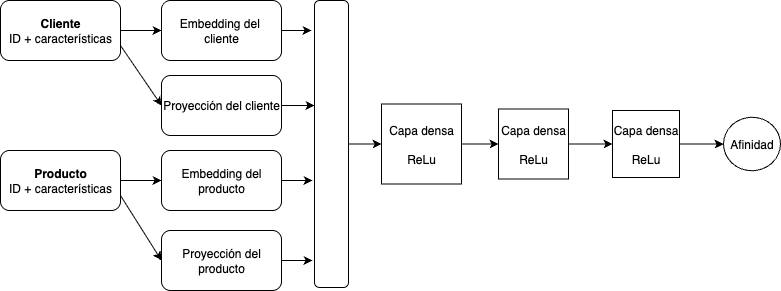
\includegraphics[scale=.5]{./Figures/ncf_hibrido.png}
	\caption{Arquitectura del modelo \textit{Neural Collaborative Filtering} híbrido.}
	\label{fig:ncf_hibrido}
\end{figure}

Durante el entrenamiento, se exploraron diferentes configuraciones de hiperparámetros, incluyendo la dimensión de los embeddings, la cantidad y tamaño de las capas ocultas, la tasa de aprendizaje y la proporción de muestreo negativo. El objetivo fue maximizar el área bajo la curva ROC-AUC sobre un conjunto de validación temporal, buscando un equilibrio entre capacidad predictiva y eficiencia computacional.

El modelo resultante produce un puntaje continuo de afinidad $\hat{y}_{ij}$ para cada combinación cliente–producto. A partir de estos valores se generan listas \textit{Top-$K$} personalizadas, ordenando los productos de mayor a menor probabilidad de interés. Este enfoque híbrido combina la expresividad de las redes neuronales con la capacidad de generalización de los sistemas de recomendación basados en contenido, ofreciendo una mayor flexibilidad para capturar interacciones complejas y atenuar los efectos del arranque en frío.

%----------------------------------------------------------------------------------------

\section{Implementación}

La implementación del sistema de recomendación requirió articular los distintos componentes desarrollados dentro de un flujo de trabajo unificado, reproducible y escalable. Para ello se diseñó un \textit{pipeline} modular que integra los procesos de ingestión, transformación, modelado y evaluación, con soporte para el versionado y monitoreo de artefactos en producción.

\subsection{Diseño del pipeline de procesamiento}

El flujo completo se estructuró en cuatro etapas principales: ingestión, preparación, modelado y predicción.  
En la fase de ingestión se integraron las fuentes de datos transaccionales, digitales y contextuales en un entorno distribuido, garantizando la consistencia de los identificadores y la alineación temporal entre registros. 

Durante la preparación, se aplicaron las transformaciones de limpieza, agregación, codificación y normalización para construir la matriz cliente–producto que sirve de insumo a los modelos.

En la etapa de modelado, se ejecutaron los distintos enfoques desarrollados, almacenando sus métricas, parámetros y versiones.

Finalmente, en la fase de predicción se generaron los puntajes de afinidad y las listas \textit{Top-$K$} para cada cliente, que constituyen la salida principal del sistema.

\subsection{Integración con la infraestructura tecnológica}

La ejecución del pipeline se realizó en la plataforma \texttt{Databricks} \cite{ARTICLE:Databricks}, que permitió procesar grandes volúmenes de datos de forma distribuida utilizando \texttt{PySpark}. Este entorno facilitó la orquestación de tareas, la paralelización de los cálculos y la trazabilidad de los resultados.  

Para la gestión del ciclo de vida de los modelos se empleó \texttt{MLflow} \cite{ARTICLE:MLflow2018}, herramienta que permitió registrar los experimentos, almacenar los parámetros y métricas, y versionar los artefactos generados durante el entrenamiento. Cada ejecución de modelo quedó asociada a un identificador único, lo que posibilita reproducir resultados, comparar configuraciones y recuperar versiones históricas de los modelos entrenados.  

Esta integración entre Databricks y MLflow conformó una infraestructura robusta y escalable, adecuada tanto para la experimentación iterativa como para la implementación de pipelines automatizados.

\subsection{Estrategias de versionado y monitoreo}

Con el fin de garantizar la trazabilidad del sistema, se adoptaron prácticas de control de versiones y monitoreo continuo.  

El código fuente y los scripts asociados al pipeline se gestionaron mediante \texttt{GitHub} \cite{ARTICLE:GitHub}, lo que permitió organizar el desarrollo de manera colaborativa y mantener un historial de cambios documentado.  

Por otro lado, los modelos registrados en \texttt{MLflow} se acompañaron de sus métricas de validación y fecha de generación, posibilitando un seguimiento temporal de su desempeño.  

Además, se establecieron controles de consistencia sobre los datos de entrada y validaciones automáticas del formato de salida, asegurando la estabilidad operativa del sistema en cada ejecución.  

En conjunto, esta arquitectura permitió implementar un flujo de trabajo integrado, auditable y escalable, garantizando la reproducibilidad de los resultados y sentando las bases para la futura incorporación de componentes en producción.


% \definecolor{mygreen}{rgb}{0,0.6,0}
% \definecolor{mygray}{rgb}{0.5,0.5,0.5}
% \definecolor{mymauve}{rgb}{0.58,0,0.82}

% %%%%%%%%%%%%%%%%%%%%%%%%%%%%%%%%%%%%%%%%%%%%%%%%%%%%%%%%%%%%%%%%%%%%%%%%%%%%%
% % parámetros para configurar el formato del código en los entornos lstlisting
% %%%%%%%%%%%%%%%%%%%%%%%%%%%%%%%%%%%%%%%%%%%%%%%%%%%%%%%%%%%%%%%%%%%%%%%%%%%%%
% \lstset{ %
%   backgroundcolor=\color{white},   % choose the background color; you must add \usepackage{color} or \usepackage{xcolor}
%   basicstyle=\footnotesize,        % the size of the fonts that are used for the code
%   breakatwhitespace=false,         % sets if automatic breaks should only happen at whitespace
%   breaklines=true,                 % sets automatic line breaking
%   captionpos=b,                    % sets the caption-position to bottom
%   commentstyle=\color{mygreen},    % comment style
%   deletekeywords={...},            % if you want to delete keywords from the given language
%   %escapeinside={\%*}{*)},          % if you want to add LaTeX within your code
%   %extendedchars=true,              % lets you use non-ASCII characters; for 8-bits encodings only, does not work with UTF-8
%   %frame=single,	                % adds a frame around the code
%   keepspaces=true,                 % keeps spaces in text, useful for keeping indentation of code (possibly needs columns=flexible)
%   keywordstyle=\color{blue},       % keyword style
%   language=[ANSI]C,                % the language of the code
%   %otherkeywords={*,...},           % if you want to add more keywords to the set
%   numbers=left,                    % where to put the line-numbers; possible values are (none, left, right)
%   numbersep=5pt,                   % how far the line-numbers are from the code
%   numberstyle=\tiny\color{mygray}, % the style that is used for the line-numbers
%   rulecolor=\color{black},         % if not set, the frame-color may be changed on line-breaks within not-black text (e.g. comments (green here))
%   showspaces=false,                % show spaces everywhere adding particular underscores; it overrides 'showstringspaces'
%   showstringspaces=false,          % underline spaces within strings only
%   showtabs=false,                  % show tabs within strings adding particular underscores
%   stepnumber=1,                    % the step between two line-numbers. If it's 1, each line will be numbered
%   stringstyle=\color{mymauve},     % string literal style
%   tabsize=2,	                   % sets default tabsize to 2 spaces
%   title=\lstname,                  % show the filename of files included with \lstinputlisting; also try caption instead of title
%   morecomment=[s]{/*}{*/}
% }


%----------------------------------------------------------------------------------------
%	SECTION 1
%----------------------------------------------------------------------------------------
% \section{Análisis del software}
 
% La idea de esta sección es resaltar los problemas encontrados, los criterios utilizados y la justificación de las decisiones que se hayan tomado.

% Se puede agregar código o pseudocódigo dentro de un entorno lstlisting con el siguiente código:

% \begin{verbatim}
% \begin{lstlisting}[caption= "un epígrafe descriptivo"]
% 	las líneas de código irían aquí...
% \end{lstlisting}
% \end{verbatim}

% A modo de ejemplo:

% \begin{lstlisting}[label=cod:vControl,caption=Pseudocódigo del lazo principal de control.]  % Start your code-block

% #define MAX_SENSOR_NUMBER 3
% #define MAX_ALARM_NUMBER  6
% #define MAX_ACTUATOR_NUMBER 6

% uint32_t sensorValue[MAX_SENSOR_NUMBER];		
% FunctionalState alarmControl[MAX_ALARM_NUMBER];	//ENABLE or DISABLE
% state_t alarmState[MAX_ALARM_NUMBER];						//ON or OFF
% state_t actuatorState[MAX_ACTUATOR_NUMBER];			//ON or OFF

% void vControl() {

% 	initGlobalVariables();
	
% 	period = 500 ms;
		
% 	while(1) {

% 		ticks = xTaskGetTickCount();
		
% 		updateSensors();
		
% 		updateAlarms();
		
% 		controlActuators();
		
% 		vTaskDelayUntil(&ticks, period);
% 	}
% }
% \end{lstlisting}



